%%%%%%%%%%%%%%%%%%%%%%%%%%%%%%%%%%%%%%%% Klasse Festlegen
%\documentclass[Master,MDS,english,fhCitStyle,HARVARD]{BASE/twbook} 
\documentclass[Master,MDS,english]{BASE/twbook} % FH definierte Zitierstandards verwenden 
%%%%%%%%%%%%%%%%%%%%%%%%%%%%%%%%%%%%%%%% Verwendete Packages
\usepackage[utf8]{inputenc} % Zeichen-Enkodierung (evtl. Abweichungen für Apple)
\usepackage[T1]{fontenc}    % Zeichen-Enkodierung
\usepackage{blindtext}      % Platzhaltertexte
\usepackage{minted}         % Darstellung von Code
\usepackage{comment}        % Auskommentieren von ganzen Passagen
\usepackage{csquotes}
\usepackage{algorithm}      % Umgebung f Algorithmen
\usepackage[noend]{algpseudocode}
                            % Wenn Sie während Ihrer Arbeit
                            % merken, dass Sie zusätzliche Funktionen
                            % benötigen ist hier ein guter Platz um
                            % weitere Packages zu laden
%%%%%%%%%%%%%%%%%%%%%%%%%%%%%%%%%%%%%%%% Zitierstil zum selbst definieren
%\usepackage[backend=biber, style=ieee]{biblatex}            % LaTeX definierter IEEE- Standard
%\usepackage[backend=biber, style=authoryear]{biblatex}      % LaTeX definierter Harvard-Standard
\usepackage{cite}
\usepackage[round]{natbib}
\usepackage{subcaption}
\captionsetup{compatibility=false}

%\addbibresource{Literatur.bib}                              % Literatur-File definieren
%%%%%%%%%%%%%%%%%%%%%%%%%%%%%%%%%%%%%%%% Einträge für Deckblatt
\title{Multi-sensor rail track detection \\ in automatic train operations}

\author{Attila Kovacs}
\studentnumber{2110854031}
%\author{Titel Vorname Name, Titel\and{}Titel Vorname Name, Titel}
%\studentnumber{XXXXXXXXXXXXXXX\and{}XXXXXXXXXXXXXXX}

\supervisor{Lukas Rohatsch}
%\supervisor[Begutachter]{Titel Vorname Name, Titel}
%\supervisor[Begutachterin]{Titel Vorname Name, Titel}
\secondsupervisor{Daniele Capriotti}
%\secondsupervisor[Begutachter]{Titel Vorname Name, Titel}
%\secondsupervisor[Begutachterinnen]{Titel Vorname Name, Titel}

\place{Wien}
%%%%%%%%%%%%%%%%%%%%%%%%%%%%%%%%%%%%%%%% Danksagung/Kurzfassung/Schlagworte
\kurzfassung{\blindtext}
\schlagworte{Deep Learning, Computer Vision, Segmentation, Automatic Train Operations}
\outline{\blindtext}
\keywords{Deep Learning, Computer Vision, Rail Track Segmentation, YOLO, Automatic Train Operations}
%\acknowledgements{\blindtext}
\setListingsAndAcronyms % Definition der Namen für Quellcodeverzeichnis 
%%%%%%%%%%%%%%%%%%%%%%%%%%%%%%%%%%%%%%%% Ende des Headers
%%%%%%%%%%%%%%%%%%%%%%%%%%%%%%%%%%%%%%%% Beginn des Dokuments
\begin{document}
%%%%%%%%%%%%%%%%%%%%%%%%%%%%%%%%%%%%%%%% 
\maketitle
%%%%%%%%%%%%%%%%%%%%%%%%%%%%%%%%%%%%%%%% Beginn des Inhalts

\chapter{Introduction} %500 words


According to the International Energy Agency (IEA), the global demand for passenger and freight transportation will more than double by 2050 compared to 2019 \citep{IEA2019}. However, a greater demand entails higher energy consumption as well as increased CO2 emissions and atmospheric pollutants.  
Given the fact that railway is one of the most efficient and reliable modes of transportation there seems to be consensus between politicians and researchers that a greater reliance of rail has the potential to counterbalance the negative impacts of transportation \citep{islam2016make, pagand2020fostering}.
The IEA lists minimizing costs per passenger-kilometer or ton-kilometer moved as one of three pillars that are essential to increase the market share of rail transportation\footnote {The other pillars are maximizing revenues from rail systems, and ensuring that all forms of transport (especially road transportation) pay not only for the use of the infrastructure they need, but also for the adverse impacts they generate.}.

Automatic Train Operations (ATO) which refers to a system that automates different aspects of train operations is expected be one of the key drivers of a more efficient and competitive railway system \citep{ERJU2019, ALSTOM2021}. ATO is estimated to reduce energy consumption by up to 45\%, increase the level of punctuality, increase operational flexibility, and allow for a 50\% better utilization of the infrastructure when combined with other technologies.

ATO relies on advanced technologies that are used to perceive and interpret the railway environment in order to allow autonomous operations with minimal or no human intervention \citep{DB2024}. 
One aspect of ATO is the precise identification and localization of railway tracks. The ability to detect and isolate tracks based on video images is essential for ensuring the safe navigation of trains through the railway network or in shunting yards. Accurate track detection ensures that the train can make informed decisions, such as adjusting speed, navigating turns, and responding to potential obstacles.

Traditional methods of track detection often rely on rule-based algorithms and image processing techniques, but these approaches may face challenges in diverse environmental conditions such as bad weather, complex background, lighting variations (e.g., day and night), and dirty cameras.
This master's thesis addresses the task of multi-sensor rail track detection in the context of ATO. We explore deep learning techniques, particularly convolutional neural networks (CNNs), that have demonstrated great success in computer vision tasks, including image segmentation. The application of deep learning to track detection is expected to outperform conventional non-AI-based techniques and thereby improving the accuracy and robustness of the system.
Our analysis is based on a multi-sensors dataset, including images of normal RGB cameras, high-resolution cameras, and infrared cameras, with different orientations, respectively. This multi-sensor approach allows to compare the the effectiveness of different cameras and informs the deployment of those in order to improve the robustness of track detection in diverse conditions. 

In the context of rail track detection, researchers have explored various areas. Yet, applying deep learning techniques to detect rail tracks is a relatively raw field. In particular, there is no research that is focusing on comparing different input images such as RGB and infrared cameras and images that are oriented to the left, center, and right of the locomotive. 
The contribution of this thesis to the literature is three-fold: First, we select and train a deep learning model capable of accurately detecting and segmenting railway tracks using data from RGB cameras, high-resolution cameras, and infrared cameras. In contrast to approaches that have been specifically tailored to the task, we apply a general framework that is easier to use by practitioners without elaborate software engineering skills.
The results of the deep learning model are compared to a non-AI based method specialized in identifying lines in images. 
Second, we conduct a comprehensive performance evaluation to assess the accuracy and computational efficiency of the proposed track detection system on images generated by different cameras.
Third, we explore the integration of the developed model into real-world applications by applying to identify tracks in video streams. 

By achieving these objectives, this research provides valuable insights and advancements to the field of railway automation, with implications for improving the safety and efficiency of automatic train operations.




\chapter{Literature review} %1000 words

Traditionally, rail track detection has been performed by first extracting features of an image (e.g., gradient-based thresholds) and then detecting rails. These approaches achieve good results in certain conditions. However, deep-learning based approaches are often more robust in real-world environments \citep{7350873, 8859360, 10.1145/3503161.3548050}.
Deep learning techniques, particularly CNNs, have emerged as powerful tools for image segmentation tasks, demonstrating success in various computer vision applications. Recent surveys on image segmentation and object detection using deep-learning techniques is provided by \cite{cmc.2023.032757} and \cite{ZAIDI2022103514}, respectively.

The following sections examine related research in track detection, considering both deep learning-based segmentation and traditional non-AI segmentation methods.



\section{Traditional rail track detection}

While deep learning has shown remarkable success in track detection, non-AI segmentation techniques continue to play a role in this field as they allow the integration of domain-specific knowledge and rules into the algorithm and require less data for training. These methods are often referred to as line segment detectors and involve traditional computer vision techniques such as thresholding, edge/contour detection, template matching, and region growing \citep{4731268, ipol.2012.gjmr-lsd, 8100103, SAHOO1988233, Mittal2022}.

\cite{5309526} present a dynamic programming algorithm to extract the rail tracks in front of the train. The idea is to first identify the vanishing point which refers to the imaginary intersection of the tracks as the distance between the tracks decreases from the bottom of the image to the top.  This step is based on computing the gradient and applying Hough transform to detect the straight lines that indicate the tracks. Next, dynamic programming is used to extract the space between the two tracks.
 \cite{qi2013efficient} apply a method based on histogram of oriented gradients (HOG) to identify tracks and switches. First, HOG features are computed;  railway tracks are then identified by a region-growing algorithm. The proposed method is able to predict the patch the train will travel by detecting the setting of the switches. 
\cite{5940410} introduce an approach that performs rail extraction by matching edge features to candidate templates.

While the previously mentioned approaches focus on images by on-board cameras, \cite{7952544} examines the detection of tracks in aerial images taken by drones. The solution approach is based on Hough transform.

\citep{rs71114916} and \citep{6783695} develop methods to recognize railroad infrastructure from 3D LIDAR data.
In \citep{rs71114916}, railway components such as rail tracks, contact cables, catenary cables, masts, and cantilevers are classified based on local neighborhood structure, shape of objects, and topological relationships among objects. 
\citep{6783695} focus on the detection of tracks. The authors utilize the geometry and reflection intensity of the tracks to
extract features and identify tracks.


\section{Deep-learning based rail track detection}

Deep-learning based techniques such as semantic segmentation incorporate convolutional neural networks (CNNs) and other deep architectures to automatically learn features from raw image data. Semantic segmentation aims to assign a label to each pixel in the image, distinguishing between the pixels that belong to the rail tracks and those that represent the background and is therefore particularly well suited for rail track detection. 

\cite{7350873} and \cite{8517865} were among the first authors who evaluated the performance of deep learning-based segmentation against traditional segmentation techniques in rail track detection. 
In \cite{7350873}, the authors propose a CNN for localizing and inspecting the condition of railway component based on gray-scale images. The authors report that the CNN model is better suited to capture complex patters compared to approaches that rely on traditional texture features (e.g., discrete Fourier transforms of local binary pattern histograms). 
\cite{8517865} detect rail tracks in aerial images by devising a CNN based approach and different traditional approaches such as thresholding. 

\cite{8859360} propose the RailNet -- a deep-learning based rail track segmentation algorithm that combines the ResNet50 backbone with a fully convolutional network. In order to train the model, the authors compile a non-public dataset consisting of 3000 images from forward-facing on-board cameras. Experiments show that RailNet is able to outperform general purpose models for segmentation.
In \cite{10.1145/3503161.3548050}, the authors compile a real-world railway dataset based on which a rail detection method referred to as Rail-Net is devised. Rail-Net outperforms traditional methods by around 51\% and other deep-learning methods by around 6\% based on accuracy when applied on the newly developed dataset. 

A machine-learning based approach is proposed by \citep{teng2016visual} where features are extracted from super-pixels (i.e., a group of adjacent pixels with similar characteristics) and classified by applying a previously trained support vector machine.


\section{Lane detection} \label{sec:lane_detection}

Lane detection for road vehicles is similar to rail track detection for locomotives in the sense that both tasks aim to identify and segment elongated shapes in complex environments that vary in lighting conditions, shadows, and occlusions. 
The field of lane detection has a rich body of literature which is among others attributed to the existence of well-established benchmark datasets such as \cite{TuSimple} and CULane \citep{pan2018SCNN}. 

Early work on lane detection is based on traditional approaches such as Hough transform and clustering \citep{10.1145/361237.361242, 5432669}. Recently, the focus of researchers has shifted to deep-learning based approaches \citep{meyer2021yolino, zheng2022clrnet, wang2022keypoint}.
\cite{tang2021review} and \cite{yang2023lane} provide comprehensive surveys on lane detection approaches. In \citep{yang2023lane}, the authors propose a combined approach in which the advantages of traditional and deep-learning based methods are mixed.


\chapter{Datasets} %2000 words

Labeled images are an essential prerequisite for training deep-learning algorithms to detect objects accurately.
With the growing popularity of deep-learning, we have observed the creation of new datasets specifically designed for railway applications.

The rail semantics dataset 2019 (RailSem19) is the first publicly available
dataset for detecting objects (including rail tracks) in the railway domain \citep{9025646}. 
The French railway signaling dataset (FRSign) is a dataset focusing only on traffic lights \citep{9025646}, whereas the Railway Pedestrian Dataset (RAWPED) is focusing on pedestrian detection methods \citep{9050835}. The dataset proposed by \cite{8859360} -- railroad segmentation dataset -- has been compiled for the development railroad segmentation algorithms but it is not available to the public. The Rail-DB dataset is available upon request \citep{10.1145/3503161.3548050}. The dataset comprises 7.432 annotated images, featuring different scenarios (e.g., weather conditions). 

This thesis is based on the first freely available multi-sensor dataset ``Open Sensor Data for Rail 2023'' (OSDaR23) for the development of fully automated driving in the railway sector \citep{DB2023, tagiew2023osdar23}.
Unlike the previously mentioned dataset that involve a limited number of sensors and perspectives, the system on the locomotive used to create the OSDaR23 dataset includes multiple infrared cameras, RGB cameras with different resolution, lidar, radar, positioning, and acceleration sensors.

Preliminary experiments indicated that our model fails to generalize when trained only on the OSDaR23 dataset due to reasons that will be described in the next section. Therefore, we also train our model on images from the RailSem19 dataset.
In the following, we give a detailed description of the two datasets used in this thesis.


\section{OSDaR23 dataset} \label{sec:OSDaR23}

\subsection{Overview}

The OSDaR23 contains 21 video sequences captured around Hamburg, Germany between 09.09.2021 and 15.09.2021 (a map of the exact locations is given in Figure~\ref{fig:map}). 
The sensor setup is very comprehensive including six RGB cameras, three
IR cameras, six lidar sensors, a 2D radar sensor, and position and acceleration sensors. In this thesis, we focus on images by RGB high resolution, RGB low resolution, and infrared sensors with three orientation (left, right, and center), respectively. One example per sensor is given in Figure~\ref{fig:sensor_image}. A detailed description of the sensors can be found in Appendix~\ref{}.

\begin{figure}[h]
\centering
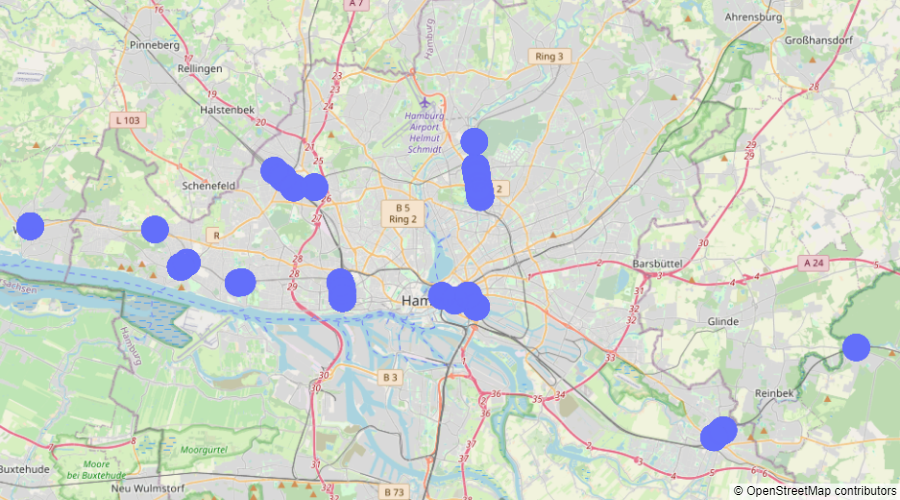
\includegraphics[width=0.5\textwidth]{images/datasets/db/map}
\caption{Locations where images were captured around Hamburg, Germany. }
\label{fig:map}
\end{figure}

\begin{figure}[h]
\centering
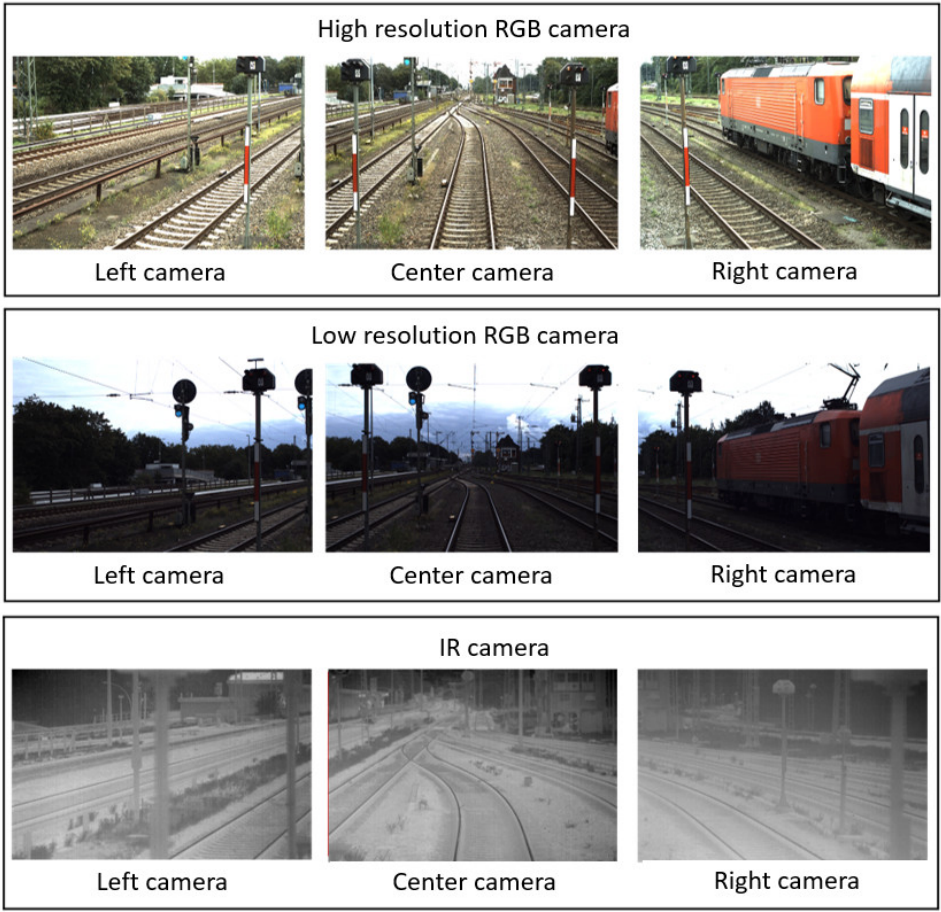
\includegraphics[width=0.5\textwidth]{images/datasets/db/2024-01-29 19_50_46-2305.03001}
\caption{Example images of high resolution RGB, low resolution RGB, and infrared sensors \citep{tagiew2023osdar23}. }
\label{fig:sensor_image}
\end{figure}


The final number of images and labels after filtering the dataset, i.e., removing images that do not contain annotated tracks, is 7.421 and 27.386, respectively. The distribution of images and labels per sensor is displayed in Figure~\ref{fig:number_images}. The size of the images is given in Table~\ref{tab:1}. Figure~\ref{fig:labels_per_image} illustrates the number of track labels per image. Most images contain track pairs. However, there are also images with odd number of tracks. The largest group are images containing one pair of tracks. Generally, the number of available images decreases as the rail network is getting more complicated.




\begin{figure}
\centering
\begin{subfigure}{.5\textwidth}
  \centering
  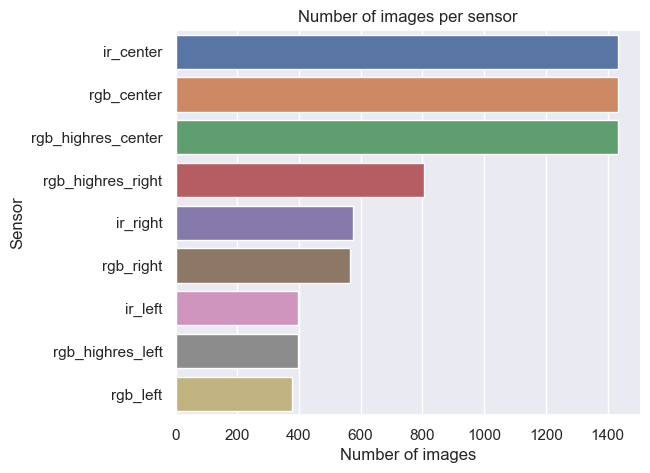
\includegraphics[width=0.9\textwidth]{images/datasets/db/images_per_sensor}
  \caption{Number of images per sensor}
  \label{fig:sub1}
\end{subfigure}%
\begin{subfigure}{.5\textwidth}
  \centering
  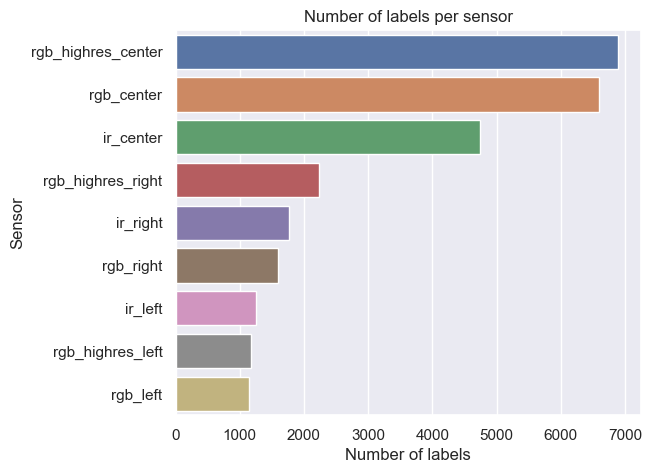
\includegraphics[width=0.9\textwidth]{images/datasets/db/labels_per_sensor}
  \caption{Number of labels per sensor}
  \label{fig:sub2}
\end{subfigure}
\caption{Number of images and labels per sensor, respectively.}
\label{fig:number_images}
\end{figure}


\begin{figure}[h]
\centering
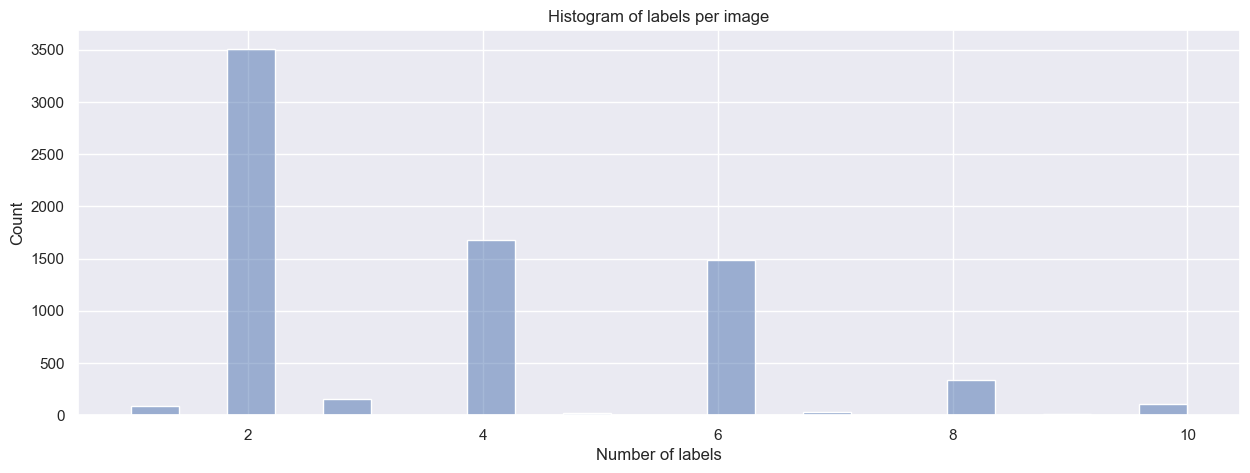
\includegraphics[width=0.9\textwidth]{images/datasets/db/labels_per_image}
\caption{Track labels per image. Most images depict track pairs. However, there are also images with odd number of tracks. }
\label{fig:labels_per_image}
\end{figure}

\begin{table}[h!]
\begin{center}
\begin{tabular}{|c| c c c|} 
  \hline
 Sensor &	Widht [px] &	Height [px] &	Aspect ration \\
 \hline
RGB low resolution &	4112 &	2504 &	1.64 \\
 \hline
RGB high resolution &	2464 &	1600 &	1.54 \\
 \hline
Infrared	& 640 &	480 &	1.33 \\
 \hline
\end{tabular}
\caption{Size of images per sensor.}
\label{tab:1}
\end{center}
\end{table}


All images were taken between 8AM and 17PM, so we cannot expect to test the effect of different sensors in the night. In particular, the RGB cameras fail to capture clear and detailed images in low-light conditions. 
Infrared cameras on the other hand, detect infrared radiation emitted by objects based on their temperature rather than visible light and are, therefore, used in low-light conditions or complete darkness\footnote{All objects with a temperature greater than absolute zero emit infrared energy.}. The thermal radiation is converted into electrical signals which are then processed to a visual image that is visible to the human eye \citep{CLARK200283}. Warmer areas are displayed as brighter, while cooler areas appear as darker shades of gray.

Emissivity, a material property that indicates how efficiently an object emits infrared radiation, plays a significant role in thermal imaging. Emissivity is measured on a scale from 0 to 1, where 0 indicates a perfect reflection of the radiation (no emission such as a mirror), and 1 indicates perfect emissivity (total emission in an object referred to as blackbody).  Detecting rail tracks in infrared images is based on the principle that polished metallic surfaces such as tracks have a low emissivity, whereas organic materials that appear often in the background have a high emissivity.  


\subsection{Brightness of the images}


In deep learning, the quality of the images can have a large impact on the efficiency. Image segmentation tasks, where the goal is to identify and classify each pixel in an image, are particularly sensitive to variations in pixel brightness and intensity.
In this section, we analyze the brightness of the images for each type of sensor. Brightness is defined as the average pixel intensity $\frac{1}{N} \sum_{i=1}^{N} I_i $; $N$ is the number of pixels in the image, and $I_i$ is the intensity of pixel $i$. In Figure~\ref{fig:brightness} shows a series of box plots with brightness values per sensor.


\begin{figure}[h]
\centering
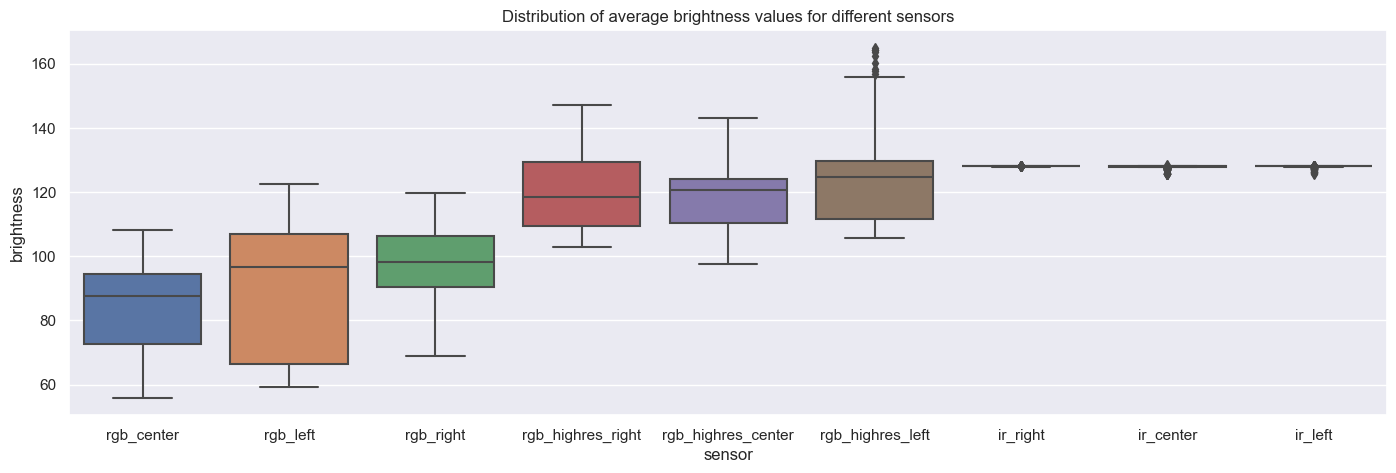
\includegraphics[width=0.9\textwidth]{images/datasets/db/brightness}
\caption{Brightness of images by sensor. }
\label{fig:brightness}
\end{figure}


Among the three types of sensors, low resolution RGB cameras produce the darkest images (a black image has a value of 0, a white image has a value of 255). 
High resolution images are brighter on average, which can be explained by different exposure settings such as shutter speed and ISO sensitivity. Both low and high-resolution cameras feature pixels of equal size ($3.45 \mu m$), so the amount of light per pixel is the same.
Infrared cameras produce images with almost constant brightness as the non-visible infrared image is mapped on a visible spectrum.

Figure~\ref{fig:brightness_examples} show one example of a bright and a dark image, respectively.


\begin{figure}
\centering
\begin{subfigure}{.5\textwidth}
  \centering
  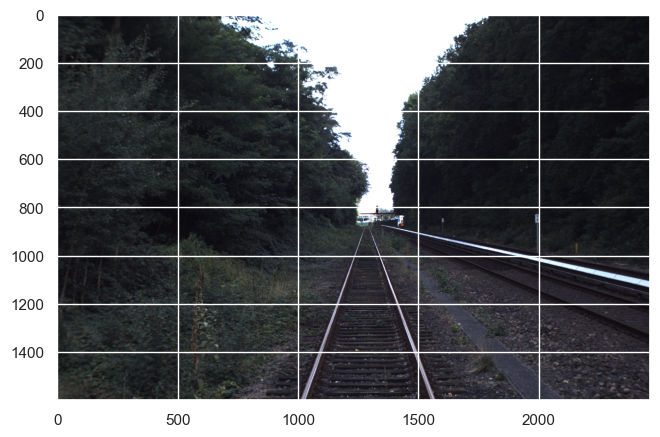
\includegraphics[width=0.9\textwidth]{images/datasets/db/dark}
  \caption{Image with low brightness value.}
%  \label{fig:sub1}
\end{subfigure}%
\begin{subfigure}{.5\textwidth}
  \centering
  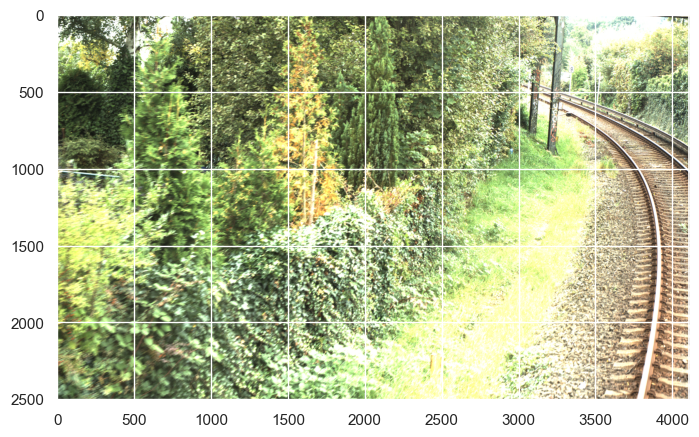
\includegraphics[width=0.9\textwidth]{images/datasets/db/bright}
  \caption{Image with high brightness value}
 % \label{fig:sub2}
\end{subfigure}
\caption{Examples of very bright and very dark image, respectively.}
\label{fig:brightness_examples}
\end{figure}



\subsection{Entropy of the images}


Shannon entropy is a measure from information theory that reflects the uncertainty or randomness associated with a set of data \citep{6773024}. In the context of images, Shannon entropy can be used to quantify the complexity in the pixel values of an image. A high entropy value indicates higher complexity or randomness in the pixel values, while a low entropy value suggests more homogeneity. \cite{rahane2020measures} report a positive correlation between the entropy of the training data and the performance of semantic segmentation tasks, highlighting that more complex images are harder to learn by deep-learning networks.
The Shannon entropy for a grayscale image is given by $H(X) = -\sum_{i=1}^{n} P(x_i) \cdot \log_2(P(x_i))$, where $P(x_i)$ is the probability of occurrence of pixel $x_i$ (i.e., the number of pixels with intensity $x_i$ divided by the total number of pixels). 
A box-plot with the entropy distribution is given in Figure~\ref{fig:entropy_examples} for each sensor. The maximum entropy value is $8 = \log_2(256)$ as we convert the images to grayscale with 256 different intensity levels.


\begin{figure}[h]
\centering
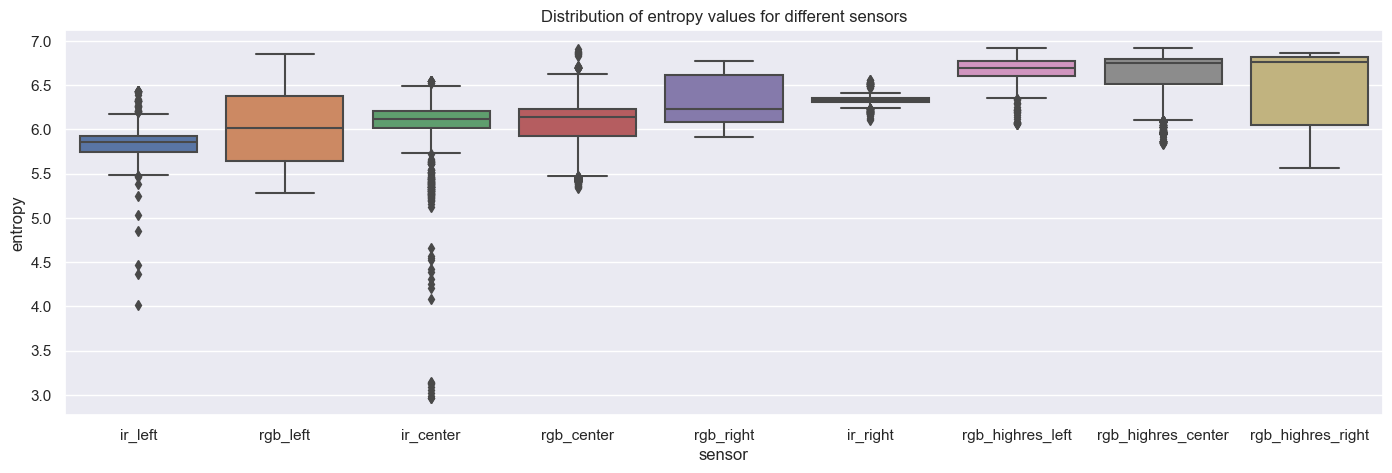
\includegraphics[width=0.9\textwidth]{images/datasets/db/entropy}
\caption{Entropy of images by sensor. }
\label{fig:entropy}
\end{figure}

Overall, the images have a high entropy -- the median values range from 5.9 to 6.8. High resolution images have the highest entropy. Infrared images do not seem to have lower entropy on average. However, certain images seem to have a very low randomness; and as it turns out also very low level of information when looking at Figure~\ref{fig:entropy_sub1}. Figure~\ref{fig:entropy_examples} highlight the visual difference between a very low and a very high entropy image.





\begin{figure}
\centering
\begin{subfigure}{.5\textwidth}
  \centering
  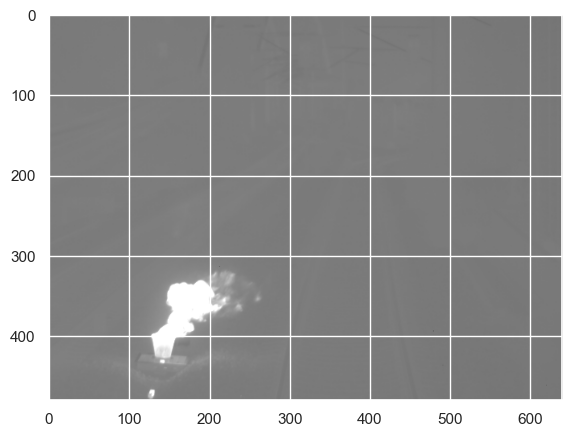
\includegraphics[width=0.9\textwidth]{images/datasets/db/low_entropy}
  \caption{Image with low entropy value.}
  \label{fig:entropy_sub1}
\end{subfigure}%
\begin{subfigure}{.5\textwidth}
  \centering
  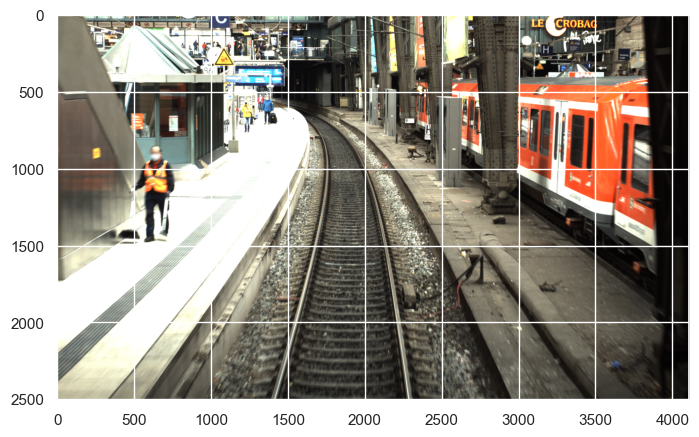
\includegraphics[width=0.9\textwidth]{images/datasets/db/high_entropy}
  \caption{Image with high entropy value}
 \label{fig:entropy_sub2}
\end{subfigure}
\caption{Examples of image with minimal and maximal entropy, respectively.}
\label{fig:entropy_examples}
\end{figure}


\subsection{Occlusion}

Certain track labels are hidden or occluded by other objects. One example is given in Figure~\ref{fig:entropy_sub2} where the train on the right covers the tracks.
In this section, we analyze the occlusion of the labels and examine those occlusions visually.

Figure~\ref{fig:occul_hist} shows the number of labels with a given occlusion level. Most of the labels, 20.069, are not occluded at all or have only a slight occlusion. However, 320 labels in 196 images are marked with an occlusion level of 100\%. Figure~\ref{fig:occlusion_examples} shows two examples where the track labels are fully covered.


\begin{figure}[h]
\centering
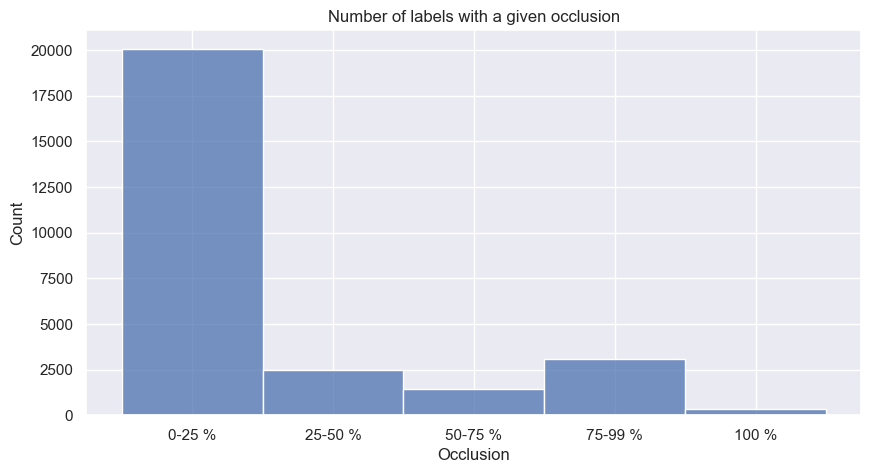
\includegraphics[width=0.9\textwidth]{images/datasets/db/occlusion_hist}
\caption{Histogram showing the occlusion level for track labels. }
\label{fig:occul_hist}
\end{figure}



We keep all images in the dataset as the CNN might recognize that there has to be a track below a train and because most images with covered labels have visible labels as well.


\begin{figure}
\centering
\begin{subfigure}{.5\textwidth}
  \centering
  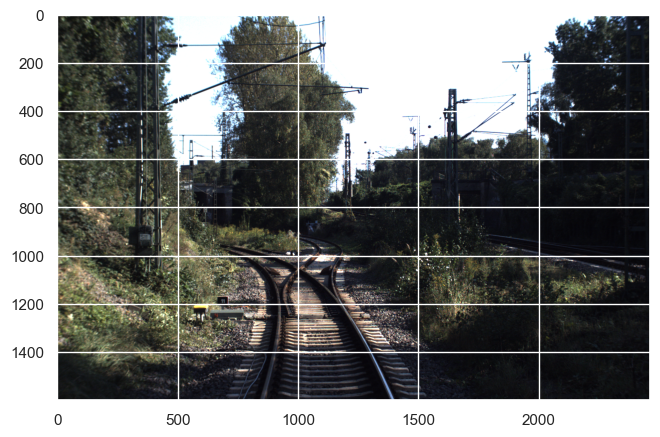
\includegraphics[width=0.9\textwidth]{images/datasets/db/occlusion_example1}
  \caption{Track on the right is hard to recognize due to poor lighting condition.}
\end{subfigure}%
\begin{subfigure}{.5\textwidth}
  \centering
  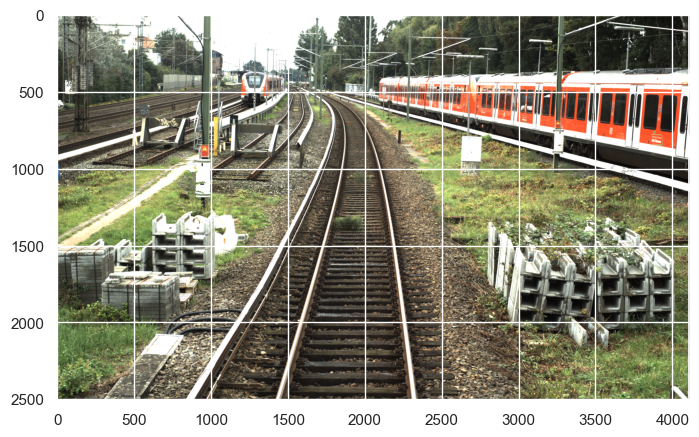
\includegraphics[width=0.9\textwidth]{images/datasets/db/occlusion_example2}
  \caption{Track is covered by train \\ on the right. }
\end{subfigure}
\caption{Examples of track labels with 100\% occlusion.}
\label{fig:occlusion_examples}
\end{figure}


\subsection{Images and video frames}

The rail tracking systems aim to analyze video streams by treating each video frame as an independent image. Consequently, the images in the OSDaR23 dataset represent individual frames extracted from video sequences. 	Figure~\ref{fig:video} shows three examples of video sequences with seven frames each. It is clear to see that there is only minor variation in the images.


\begin{figure}
\centering
\begin{subfigure}{\textwidth}
  \centering
  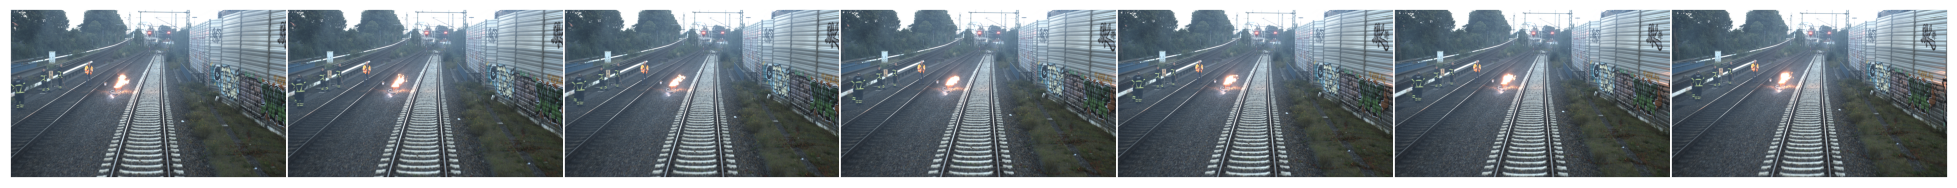
\includegraphics[width=0.9\textwidth]{images/datasets/db/video_1}
  \label{fig:sub1}
\end{subfigure}%
\vskip\baselineskip
\begin{subfigure}{\textwidth}
  \centering
  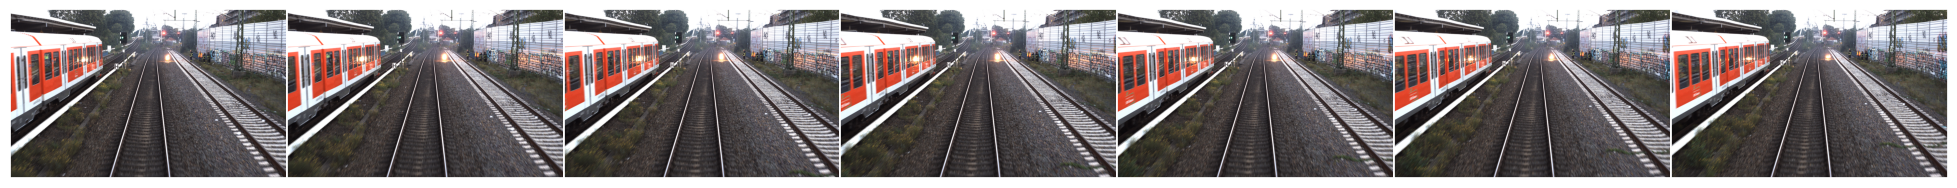
\includegraphics[width=0.9\textwidth]{images/datasets/db/video_2}
  \label{fig:sub2}
\end{subfigure}
\vskip\baselineskip
\begin{subfigure}{\textwidth}
  \centering
  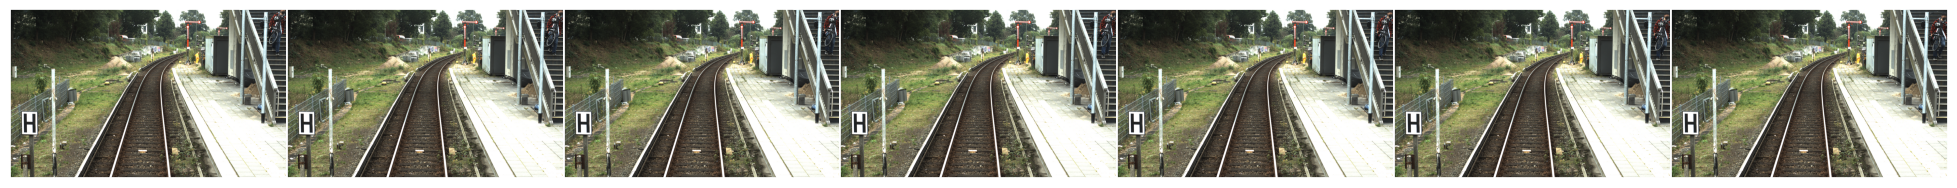
\includegraphics[width=0.9\textwidth]{images/datasets/db/video_3}
  \label{fig:sub3}
\end{subfigure}
\caption{Three examples with seven video frames (i.e., images), respectively.}
\label{fig:video}
\end{figure}


Two major issues when training a model on a dataset that consists of similar images is a lack of generalization (i.e., inability to generalize well on diverse and unseen images) and reduced robustness (i.e., vulnerability to variations in lighting conditions and backgrounds). 
In order to mitigate the issues, we add images from the RailSem19 dataset to the training data.




\section{RailSem19 dataset}

The RailSem19 dataset \citep{9025646} is not the primary focus on of this thesis. However, the previous analysis reveals that among the 7,421 images within the OSDaR23 dataset, a significant number show high similarity. This similarity is due to the fact that the images are frames from a video sequence and the presence of three cameras for each orientation, respectively.
The RailSem19 dataset is added to the training set in order to increase the performance of the segmentation approach.
In the following, we will examine the RailSem19 dataset in more detail.

The dataset consists of 8500 rail images, taken in different countries, and weather and lighting conditions. The number of rail annotations is 58.483. All images have a size of 1920x1080 pixels. 
Figure~\ref{fig:labels_per_image_railsem} shows a histogram of images with the respective number of track labels. Most images contain 4 track labels (i.e., two pairs of tracks) but the dataset also contains complicated networks with 26 pairs of tracks. An example of a simple and an example of a complicated infrastructure is given in Figure~\ref{fig:railsem_complicated_vs_simple}.



\begin{figure}[h]
\centering
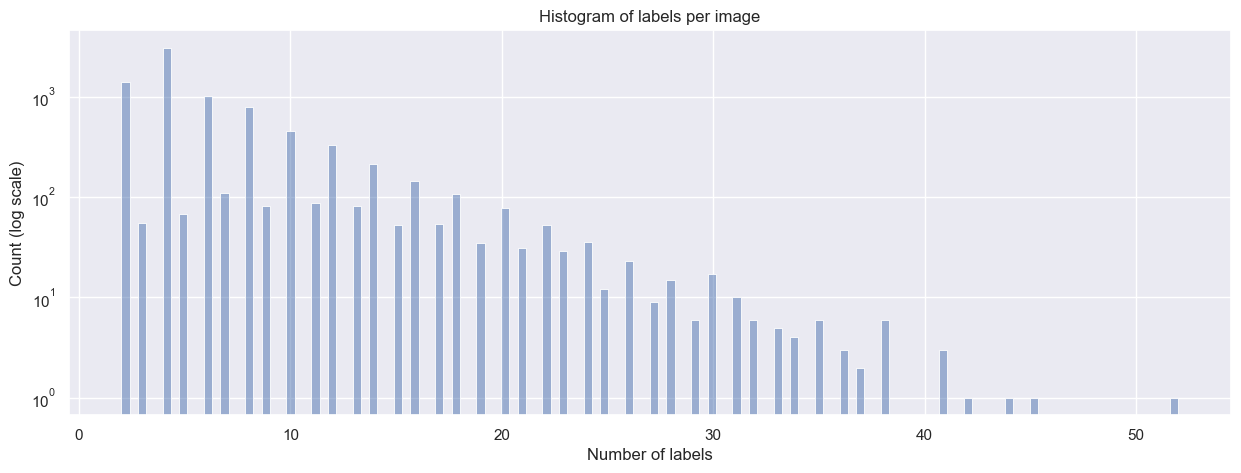
\includegraphics[width=0.9\textwidth]{images/datasets/railsem/labels_per_image}
\caption{Track labels per image on a logarithmic scale. The images range from simple railroads with a single pair of tracks to complicated networks with 26 pairs of tracks. }
\label{fig:labels_per_image_railsem}
\end{figure}


\begin{figure}
\centering
\begin{subfigure}{.5\textwidth}
  \centering
  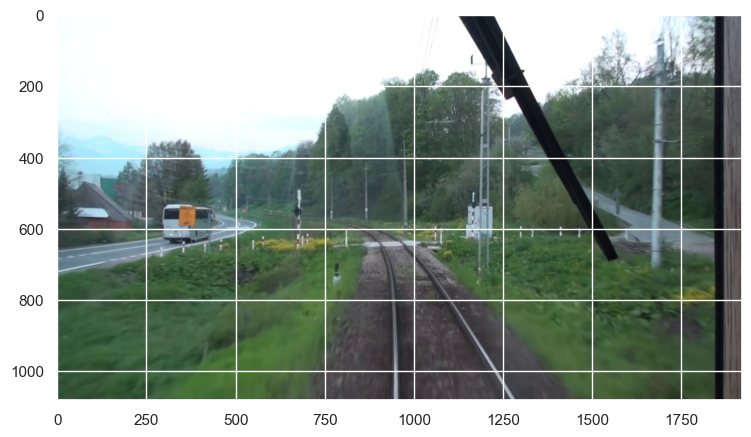
\includegraphics[width=0.9\textwidth]{images/datasets/railsem/example_2_tracks}
  \caption{Simple rail infrastructure.}
\end{subfigure}%
\begin{subfigure}{.5\textwidth}
  \centering
  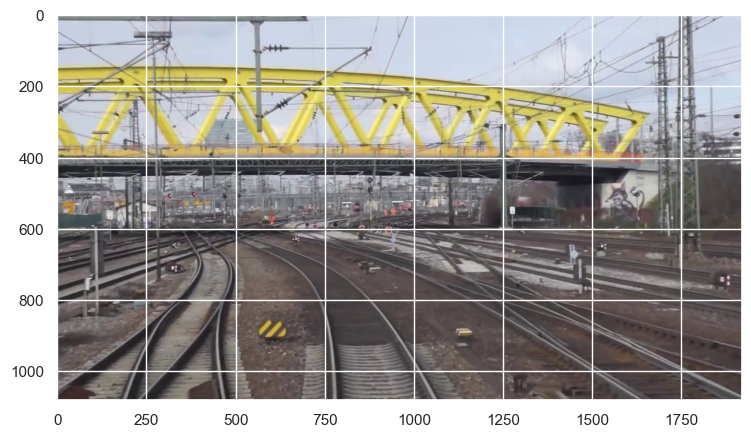
\includegraphics[width=0.9\textwidth]{images/datasets/railsem/example_52_tracks}
  \caption{Complicated rail infrastructure. }
\end{subfigure}
\caption{Examples of simple and complicated rail infrastructure.}
\label{fig:railsem_complicated_vs_simple}
\end{figure}


Figure~\ref{fig:railsem_brightness} and  Figure~\ref{fig:railsem_entropy} show the distribution of the brightness values and the entropy values as defined in Section~\ref{sec:OSDaR23}, respectively. The RailSem19 images are mostly brighter than the OSDaR23; the distribution of the values ranges from almost black images to almost white images (see Figure~\ref{fig:railsem_sub1} and Figure~\ref{fig:railsem_sub1}). The entropy of the RailSem19 images is similar to the images in the OSDaR23 dataset. The outliers at the lower end of the entropy spectrum are associated with infrared images in the OSDaR23 dataset. Howerver, in RailSem19 low entropy images are often images that were generated in tunnels or at night. Figure~\ref{fig:railsem_sub2} and Figure~\ref{fig:railsem_sub4}) are images with a low entropy levels close to zero whereas Figure~\ref{fig:railsem_sub4}) has the highest entropy level in the data set with a score of 6.97.


\begin{figure}
\centering
\begin{subfigure}{.5\textwidth}
  \centering
  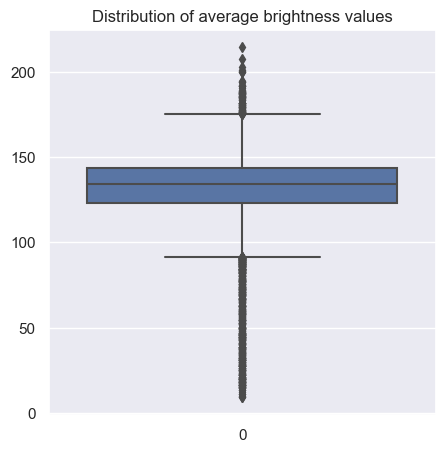
\includegraphics[width=0.9\textwidth]{images/datasets/railsem/brightness}
  \caption{Boxplot of brightness values.}
   \label{fig:railsem_brightness}
\end{subfigure}%
\begin{subfigure}{.5\textwidth}
  \centering
  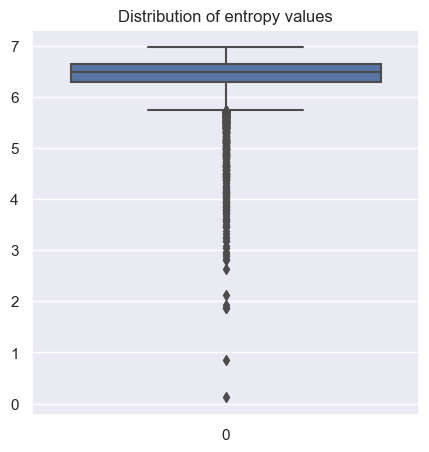
\includegraphics[width=0.9\textwidth]{images/datasets/railsem/entropy}
  \caption{Boxplot of entropy values. }
  \label{fig:railsem_entropy}
\end{subfigure}
\caption{Brightness and entropy of RailSem19 images.}
\label{fig:railsem_brightness_entropy}
\end{figure}




\begin{figure}
\centering
\begin{subfigure}{.5\textwidth}
  \centering
  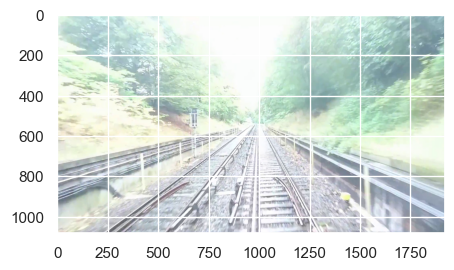
\includegraphics[width=0.9\textwidth]{images/datasets/railsem/example_bright}
  \caption{Bright image.}
  \label{fig:railsem_sub1}
\end{subfigure}%
\begin{subfigure}{.5\textwidth}
  \centering
  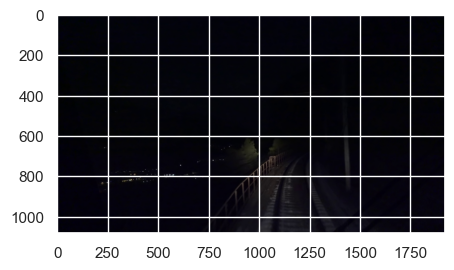
\includegraphics[width=0.9\textwidth]{images/datasets/railsem/example_dark}
  \caption{Dark image.}
  \label{railsem_sub2}
\end{subfigure}
\vskip\baselineskip
\begin{subfigure}{.5\textwidth}
  \centering
  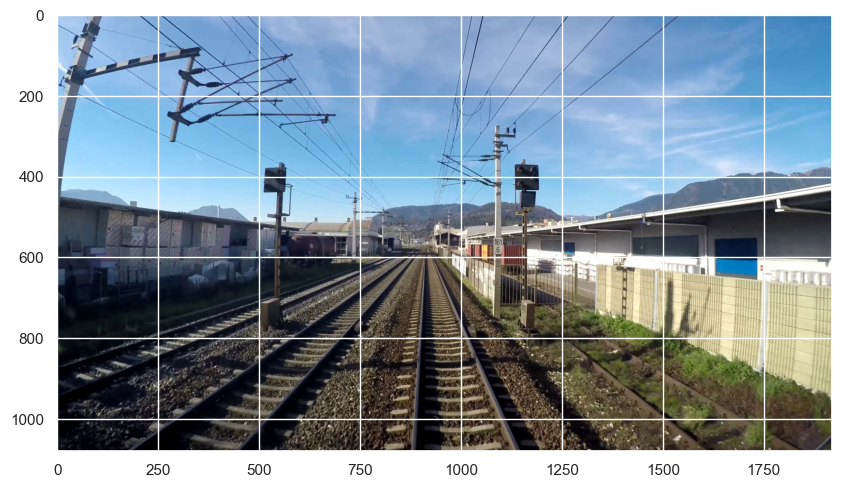
\includegraphics[width=0.9\textwidth]{images/datasets/railsem/example_high_entropy}
  \caption{High entropy.}
  \label{railsem_sub3}
\end{subfigure}%
\begin{subfigure}{.5\textwidth}
  \centering
  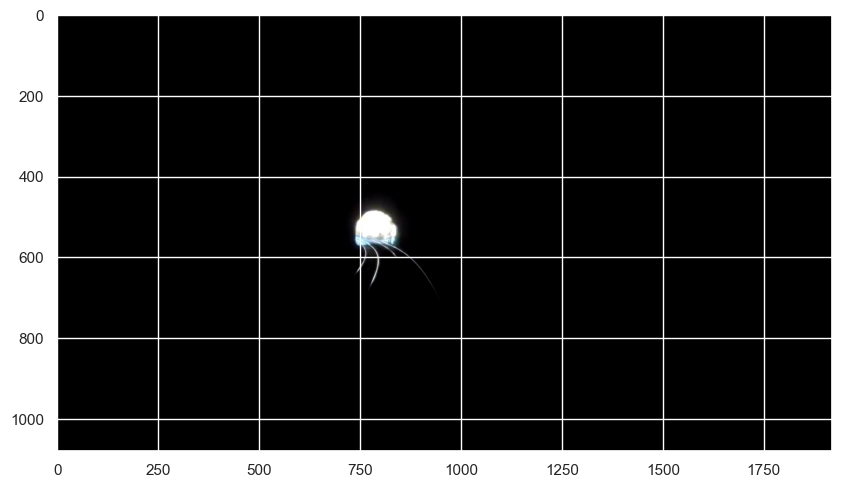
\includegraphics[width=0.9\textwidth]{images/datasets/railsem/example_low_entropy}
  \caption{Low entropy.}
  \label{railsem_sub4}
\end{subfigure}
\caption{Extreme examples with regard to brightness and entropy.}
\label{fig:examples}
\end{figure}


\section{Data splitting}

Splitting a dataset into training, validation, and test sets is a standard practice in machine learning to evaluate and improve the performance of a model. 
 Separating data into distinct sets and using them at different stages of development, prevents unintended data leakage where information from the test or validation set influences the training process.
 
 The validation set assesses performance during training, refines hyperparameters, and guards against overfitting. Adjustments made based on validation set evaluations ensure the model generalizes effectively to new, unseen data. 

The training set is used to train the model -- the model learns patterns and relationships within the training data.
The validation set is used to evaluate the performance during the training process, fine-tune the hyperparameters of the model, and to prevent overfitting (i.e., a situation when a model performs well on the training data but fails to generalize to new data). We can make adjustments to the algorithm and optimize the performance on the validation set without compromising the model's ability to generalize to new data. 
The test set is reserved for the final evaluation of the model. The test set allows for an unbiased assessment of the model's performance on data it has never seen before and provides, therefore, an estimate of how well the model is likely to perform on new, real-world data.

Our approach is to perform a random split with a share of 70\%/15\%/15\% for train, validation, and test set respectively. Splitting the RailSem19 set is straightforward; we randomly assign images to each set resulting in 5.950, 1.275, and 1.275 images per set, respectively. However, the OSDaR23 comprises many images with high similar (e.g., frames from a video that was take when the locomotive was standing still), so we perform a random split not on individual images but on videos sequences. The approach results in 5.506 images for training, 987 images for validation, and 928 images for testing.
The assignment of video sequences to the respective set and the split on sensor level is given in Appendix~\ref{app:data_split}



\chapter{Solution approach and experiments} % 4000 words

Given an image captured by an on-board camera on the locomotive, our objective is to precisely delineate the visible rail tracks. The output is  a polyline describing each track.

\cite{meyer2021yolino} introduce YOLinO, a versatile and efficient algorithm inspired by single-shot object detection. It is designed to detect polylines in the context of lane detection, as discussed in Section~\ref{sec:lane_detection}. While the proposed approach is suitable for rail track detection, adapting the existing codebase from lane detection to rail track detection exceeds the scope of this thesis. Furthermore, our goal is to employ an off-the-shelf solution framework that can be readily utilized by a broader audience.


Within computer vision, semantic segmentation is a well-studied domain focusing on classifying each pixel in an image into predefined categories \citep{MO2022626}. Conceptually, it 
can be seen as an extension of object detection, a technique that recognizes and precisely locates objects within an image using bounding boxes.
The pixel-level precision in object classification enables the understanding of the image context and is therefore often used in applications like autonomous driving and robotics.

Our approach to the rail detection problem is based on two steps. First, we perform a semantic segmentation where each pixel is classified as either rail track or background. In a second step, the result of the segmentation task is used to define one polyline for each track. Segmentation is performed by the YOLOv8 algorithm \citep{Jocher_Ultralytics_YOLO_2023}.  YOLOv8, short for "You Only Look Once, version 8," is the latest version in the YOLO series of real-time object detectors, offering state-of-the-art performance in terms of accuracy and speed \citep{ultralytics_docs}. YOLOv8 builds upon the YOLO architecture, introduced in \cite{redmon2016you} -- a paper that has received more than 43.000 citations. Since the introduction of the original YOLO in 2016, the framework has been tested extensively with remarkable results \citep{JIANG20221066, cryptography6020016, Diwan2023}. The efficiency of the YOLO implementations by \cite{Jocher_Ultralytics_YOLO_2023} for segmentation tasks is examined in \cite{agriculture13081643} and \cite{STRAKER2023100045}.






\section{Modeling and performance evaluation} 






\section{Transforming labels}









\section{Non-AI based segmentation}




\section{Deep-learning based segmentation}



\chapter{Results} % 2000 words





\chapter{Conclusion} % 500 words





Etwas Text... Hier kommen noch einige Abkürzunge vor zum Beispiel \ac{ABC},\ac{WWW} und \ac{ROFL}.


\section{Algorithms}


Use a defined environment for algorithms.

Algorithm \ref{alg:euclid} is an example from the gallery (\url{https://www.overleaf.com/latex/examples/euclids-algorithm-an-example-of-how-to-write-algorithms-in-latex/mbysznrmktqf}) .
%%%%%%%%%%%%%%%%%%%%%%%%%%%%%%%%%%%%%%%%%%%%%%%%%%%%%%%%%%%%%%%%%%
\begin{algorithm}
\caption{Euclid’s algorithm}\label{alg:euclid}
\begin{algorithmic}[1]
\Procedure{Euclid}{$a,b$}\Comment{The g.c.d. of a and b}
\State $r\gets a\bmod b$
\While{$r\not=0$}\Comment{We have the answer if r is 0}
\State $a\gets b$
\State $b\gets r$
\State $r\gets a\bmod b$
\EndWhile\label{euclidendwhile}
\State \textbf{return} $b$\Comment{The gcd is b}
\EndProcedure
\end{algorithmic}
\end{algorithm}
%%%%%%%%%%%%%%%%%%%%%%%%%%%%%%%%%%%%%%%%%%%%%%%%%%%%%%%%%%%%%%%%%% Hier beginnen die Verzeichnisse.
\clearpage                                                       % Beginne neue Seite

%\printbib                                                        % Literaturverzeichnis LaTeX-Zitier-Standard
%\printbib{Literatur}                                             % Literaturverzeichnis FH-Zitier-Standard
%\printbibliography
\bibliographystyle{plainnat} % We choose the "plain" reference style
\bibliography{Literatur} % Entries are in the refs.bib file

\clearpage

\listoffigures                                                   % Abbildungsverzeichnis
\clearpage

\listoftables                                                    % Tabellenverzeichnis
\clearpage

\listoflistings                                                  % Quellcodeverzeichnis
\clearpage

\phantomsection
\addcontentsline{toc}{chapter}{\listacroname}
\chapter*{\listacroname}
\begin{acronym}[XXXXX]
    \acro{ABC}[ABC]{Alphabet}
    \acro{WWW}[WWW]{world wide web}
    \acro{ROFL}[ROFL]{Rolling on floor laughing}
    
    
    
    \acro{ATO}[ATO]{Automatic Train Operations}
    \acro{CNN}[CNN]{Convolutional Neural Network}
    
\end{acronym}
%%%%%%%%%%%%%%%%%%%%%%%%%%%%%%%%%%%%%%%%%%%%%%%%%%%%%%%%%%%%%%%%%% Hier beginnt der Anhang.
\clearpage


\appendix
\chapter{Appendix A}

\section{Dataset split} \label{app:data_split}

Splitting the OSDaR23 dataset in to train, validation, and test subsets is performed based on video sequences. Table~\ref{tab:dataset_split} lists the assignment of sequences to the respective subset. Figure~\ref{fig:data_split} show the split on an image level in total and for each sensor type.

\begin{table}[ht]
\centering
\footnotesize
\begin{tabular}{|l|l|l|}
\hline
\textbf{Train} & \textbf{Validation} & \textbf{Test} \\
\hline
10\_station\_suelldorf\_10.1 & 16\_under\_bridge\_16.1 & 14\_signals\_station\_14.1 \\
11\_main\_station\_11.1 & 18\_vegetation\_switch\_18.1 & 21\_station\_wedel\_21.1 \\
12\_vegetation\_steady\_12.1 & 1\_calibration\_1.2 & 4\_station\_pedestrian\_bridge\_4.2 \\
13\_station\_ohlsdorf\_13.1 & 3\_fire\_site\_3.3 & 4\_station\_pedestrian\_bridge\_4.5 \\
14\_signals\_station\_14.2 & 9\_station\_ruebenkamp\_9.1 & 7\_approach\_underground\_station\_7.2 \\
14\_signals\_station\_14.3 & 9\_station\_ruebenkamp\_9.2 & 8\_station\_altona\_8.3 \\
15\_construction\_vehicle\_15.1 & & \\
17\_signal\_bridge\_17.1 & & \\
19\_vegetation\_curve\_19.1 & & \\
1\_calibration\_1.1 & & \\
20\_vegetation\_squirrel\_20.1 & & \\
21\_station\_wedel\_21.2 & & \\
21\_station\_wedel\_21.3 & & \\
2\_station\_berliner\_tor\_2.1 & & \\
3\_fire\_site\_3.1 & & \\
3\_fire\_site\_3.2 & & \\
3\_fire\_site\_3.4 & & \\
4\_station\_pedestrian\_bridge\_4.1 & & \\
4\_station\_pedestrian\_bridge\_4.3 & & \\
4\_station\_pedestrian\_bridge\_4.4 & & \\
5\_station\_bergedorf\_5.1 & & \\
5\_station\_bergedorf\_5.2 & & \\
6\_station\_klein\_flottbek\_6.1 & & \\
6\_station\_klein\_flottbek\_6.2 & & \\
7\_approach\_underground\_station\_7.1 & & \\
7\_approach\_underground\_station\_7.3 & & \\
8\_station\_altona\_8.1 & & \\
8\_station\_altona\_8.2 & & \\
9\_station\_ruebenkamp\_9.3 & & \\
9\_station\_ruebenkamp\_9.4 & & \\
9\_station\_ruebenkamp\_9.5 & & \\
9\_station\_ruebenkamp\_9.6 & & \\
9\_station\_ruebenkamp\_9.7 & & \\
\hline
\end{tabular}
\caption{Dataset split: OSDaR23 }
\label{tab:dataset_split}
\end{table}



\begin{figure}[h]
\centering
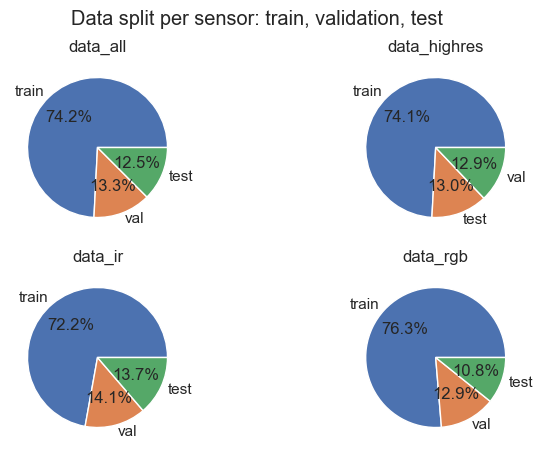
\includegraphics[width=0.9\textwidth]{images/datasets/db/data_split}
\caption{OSDaR23 data split on image level in total and on sensor level. }
\label{fig:data_split}
\end{figure}



\clearpage
\chapter{Appendix B}
\end{document}
%%%%%%%%%%%%%%%%%%%%%%%%%%%%%%%%%%%%%%%%%%%%%%%%%%%%%%%%%%%%%%%%%% Ende des Inhalts